% Preview source code

%% LyX 2.1.4 created this file.  For more info, see http://www.lyx.org/.
%% Do not edit unless you really know what you are doing.
\documentclass[12pt,english]{article}
\renewcommand{\familydefault}{\sfdefault}
\usepackage[T1]{fontenc}
\usepackage[latin9]{inputenc}
\usepackage[a4paper]{geometry}
\geometry{verbose,tmargin=25mm,bmargin=25mm,lmargin=25mm,rmargin=25mm}
\usepackage{fancyhdr}
\pagestyle{fancy}
\usepackage{color}
\usepackage{amstext}
\PassOptionsToPackage{normalem}{ulem}
\usepackage{ulem}

\makeatletter
%%%%%%%%%%%%%%%%%%%%%%%%%%%%%% User specified LaTeX commands.
\usepackage{titling, graphicx}
\usepackage{tikz}
%\usepackage{strtikz}

\usetikzlibrary{shapes,arrows.meta, intersections, graphs, graphs.standard}
\usetikzlibrary{math}

\date{}
%\setlength\parindent{0pt}

\pretitle{\begin{center} \Large \bf \vspace{-2em}}
\posttitle{\par\end{center}\vspace{-1.5em}}
\preauthor{\begin{center} \large \lineskip 1em \begin{tabular}[t]{c}}
\postauthor{\end{tabular}\par\end{center}\vspace{-5em}}

\rhead{Test}
\lhead{\thetitle}

\fancypagestyle{firststyle}
{
\lhead{None}
\chead{
\includegraphics[width=0.75cm, keepaspectratio=true]{logo.pdf}}
\rhead{None}
}

\makeatother

\usepackage{babel}





\begin{document}

\title{Testing}


\author{Test Test}

\maketitle
\thispagestyle{firststyle}


\section{Testing}


\begin{center}
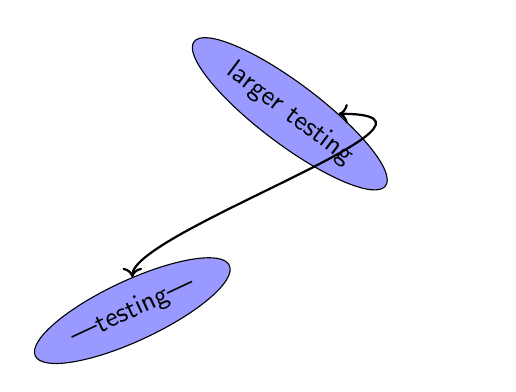
\begin{tikzpicture} [scale=0.5,fill=blue!40]
\path (0,0) node(a) [ellipse, rotate=25, draw, fill] {|testing|}
      (4,5) node(b) [ellipse, rotate=-37, draw, fill] {larger testing};
\draw[thick,<->] (a) .. controls +(up:2cm) and +(right:5cm) .. (b);

\end{tikzpicture}
\end{center}

\subsection{TestingSub}
This section explained blah blah blah...

\noindent
Testing one 2

\end{document}
